\chapter*{ПРИЛОЖЕНИЕ A}
\addcontentsline{toc}{chapter}{ПРИЛОЖЕНИЕ А}

\section*{Описание интерфейсов}

\begin{figure}[h]
	\centering
	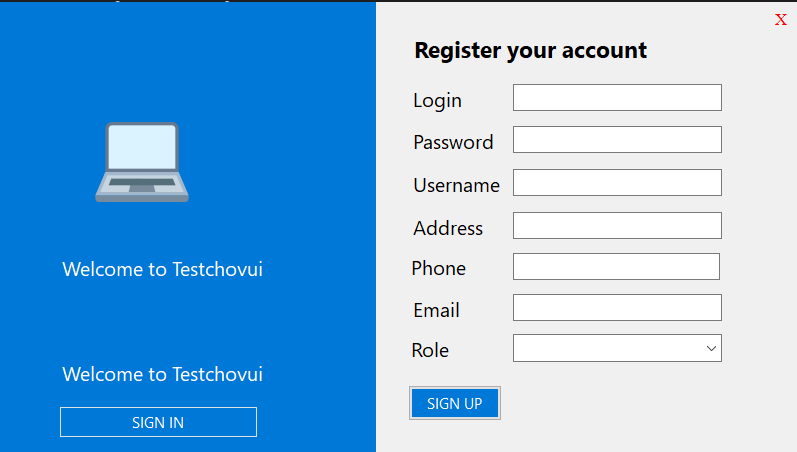
\includegraphics[height=0.2\textheight]{img/signup.png}
	\caption{Демонстрация работы программы при регистрации}
	\label{img:ex1}
\end{figure}

\begin{figure}[h]
	\centering
	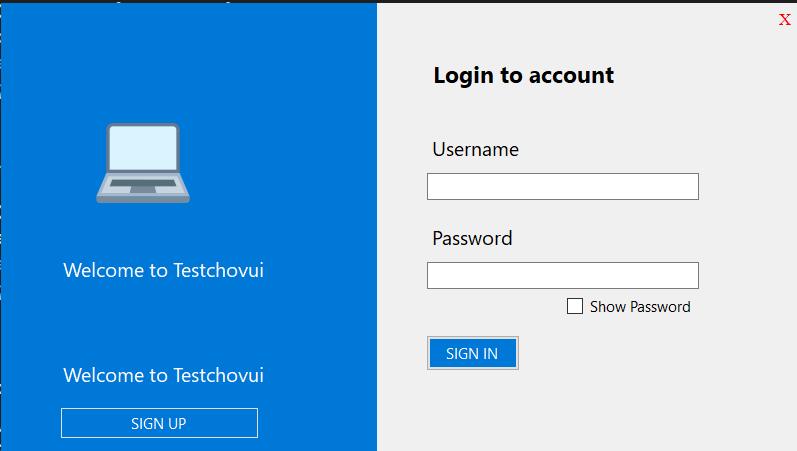
\includegraphics[height=0.2\textheight]{img/signin.png}
	\caption{Демонстрация работы программы при входе в систему}
	\label{img:ex1a}
\end{figure}




\begin{figure}[h]
	\centering
	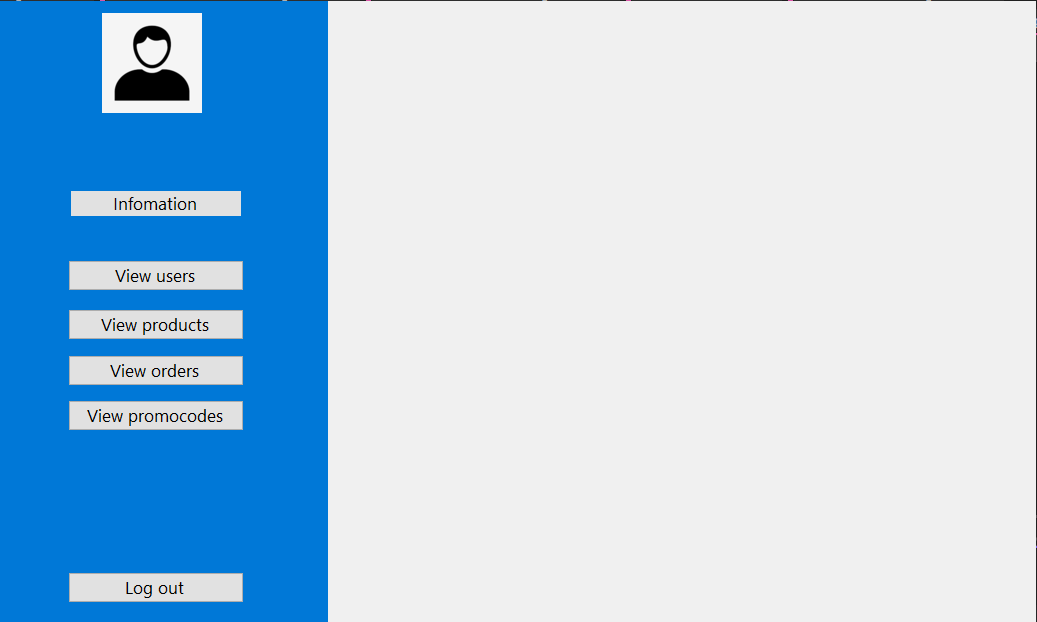
\includegraphics[height=0.4\textheight]{img/admin_0.png}
	\caption{Демонстрация главного экрана админстратора}
	\label{img:ex2}
\end{figure}

\begin{figure}[h]
	\centering
	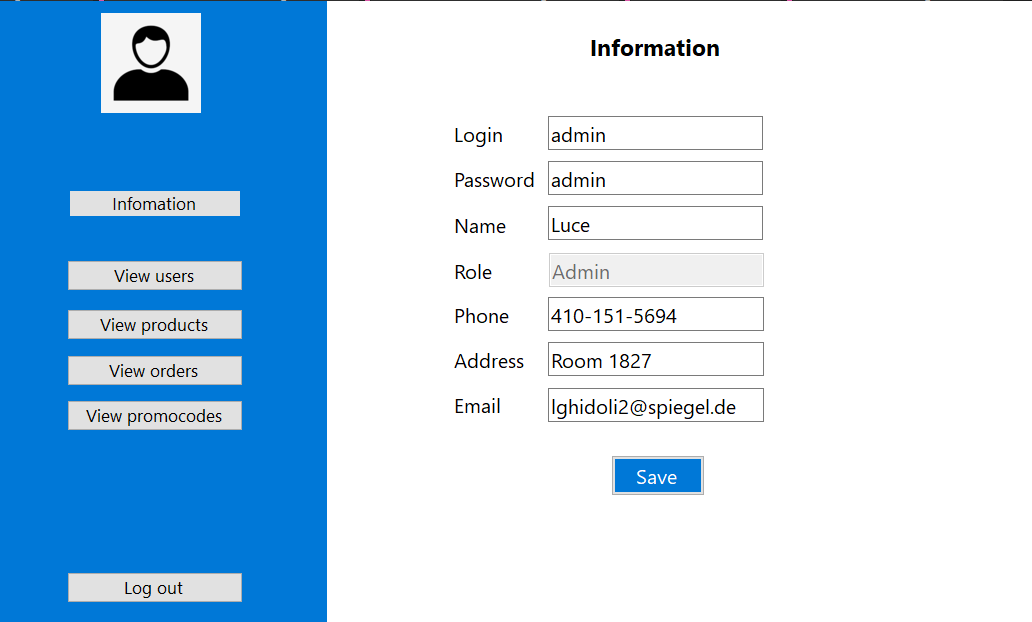
\includegraphics[height=0.4\textheight]{img/admin_1.png}
	\caption{Демонстрация экрана админстратора при просмотре информации}
	\label{img:ex3}
\end{figure}

\begin{figure}[h]
	\centering
	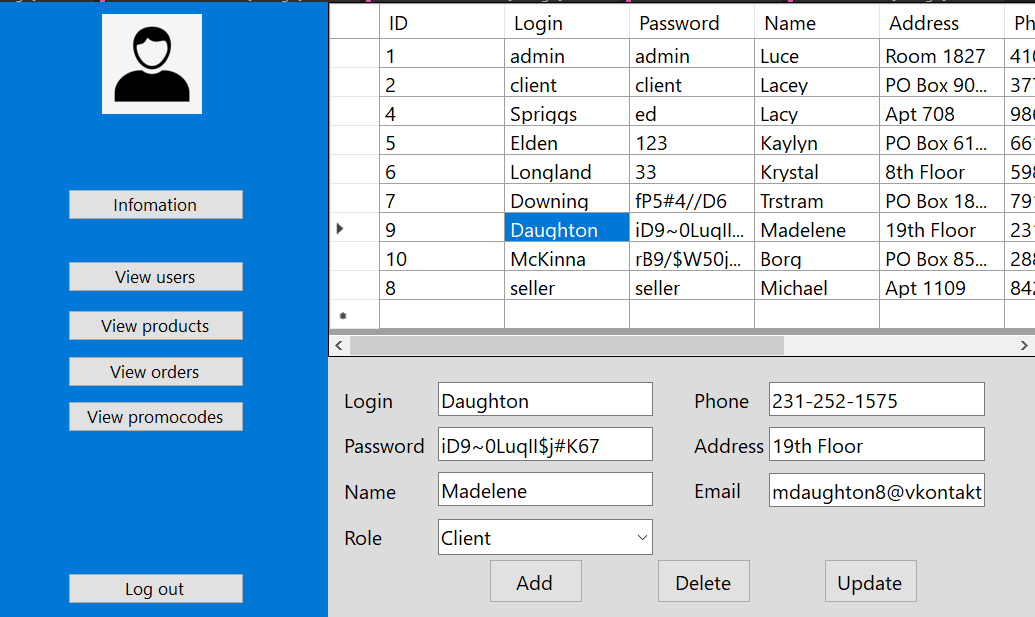
\includegraphics[height=0.4\textheight]{img/admin_2.png}
	\caption{Демонстрация экрана админстратора при просмотре пользователей}
	\label{img:ex4}
\end{figure}

\begin{figure}[h]
	\centering
	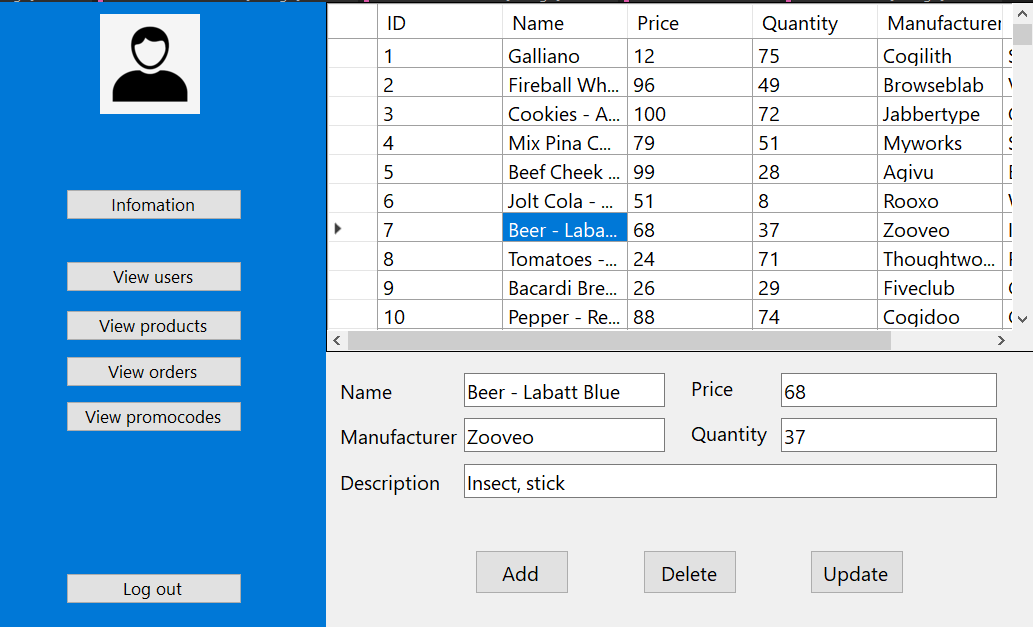
\includegraphics[height=0.4\textheight]{img/admin_5.png}
	\caption{Демонстрация экрана админстратора при просмотре товаров}
	\label{img:ex5}
\end{figure}

\begin{figure}[h]
	\centering
	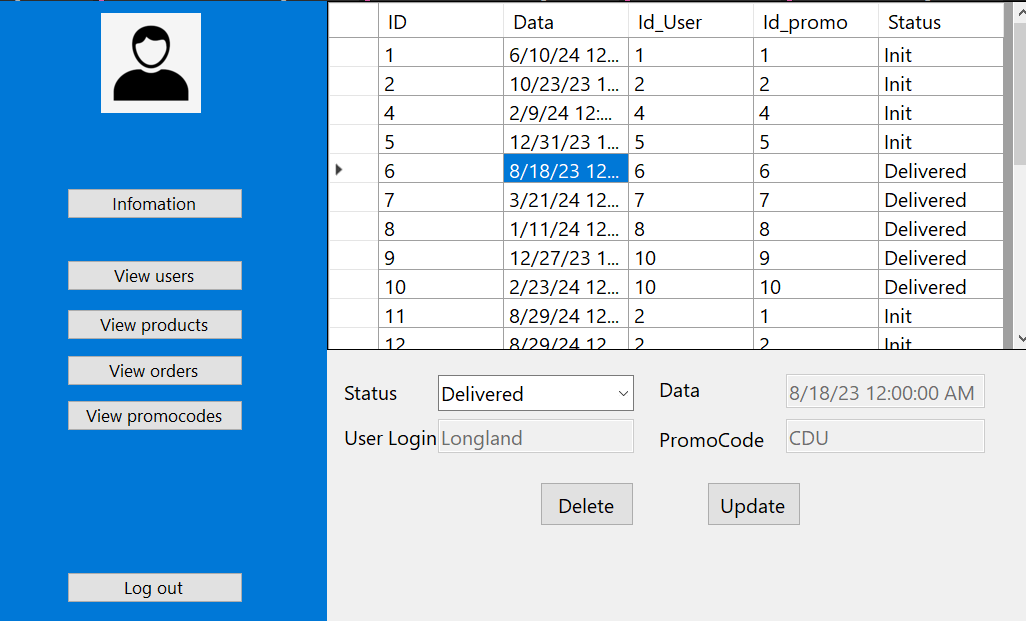
\includegraphics[height=0.4\textheight]{img/admin_3.png}
	\caption{Демонстрация экрана админстратора при просмотре заказов}
	\label{img:ex6}
\end{figure}

\begin{figure}[h]
	\centering
	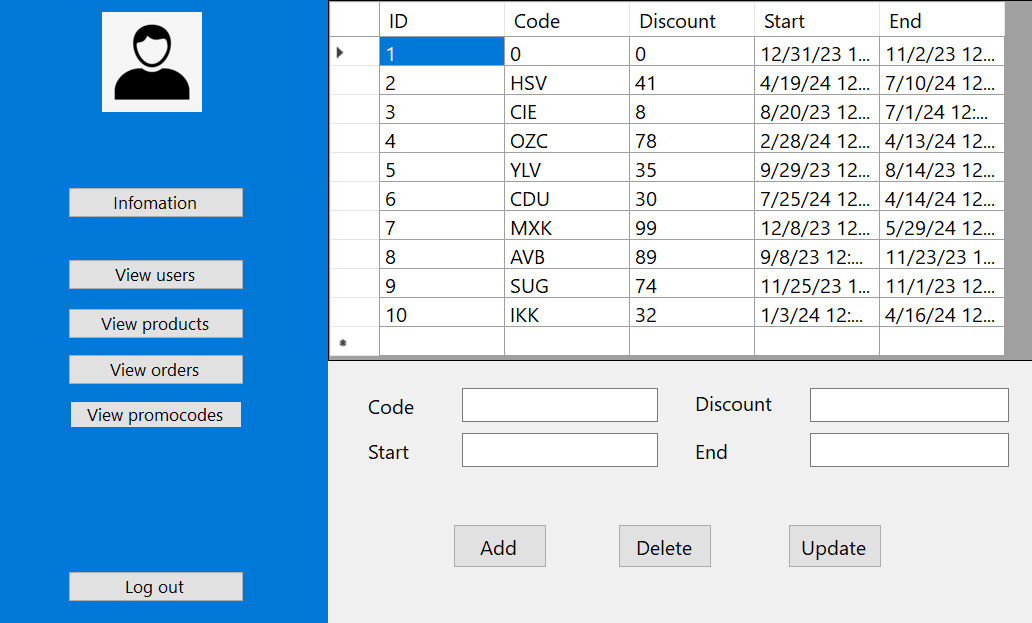
\includegraphics[height=0.4\textheight]{img/admin_4.png}
	\caption{Демонстрация экрана админстратора при просмотре промокодов}
	\label{img:ex7}
\end{figure}

\begin{figure}[h]
	\centering
	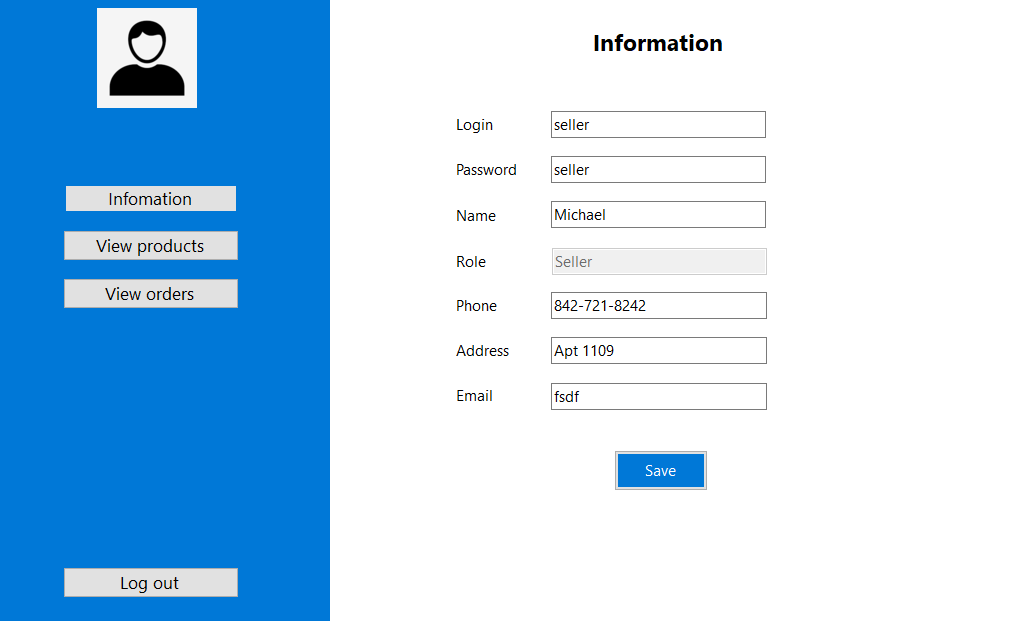
\includegraphics[height=0.4\textheight]{img/seller_0.png}
	\caption{Демонстрация главного экрана поставщика}
	\label{img:ex8}
\end{figure}

\begin{figure}[h]
	\centering
	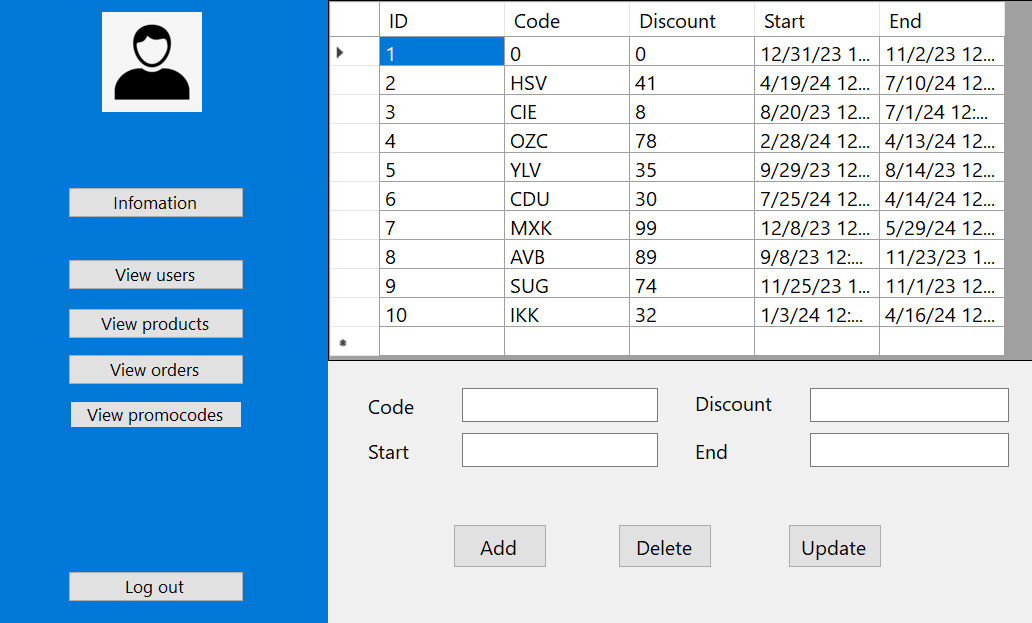
\includegraphics[height=0.4\textheight]{img/admin_4.png}
	\caption{Демонстрация экрана клиентов при просмотре корзины}
	\label{img:ex9}
\end{figure}

\begin{figure}[h]
	\centering
	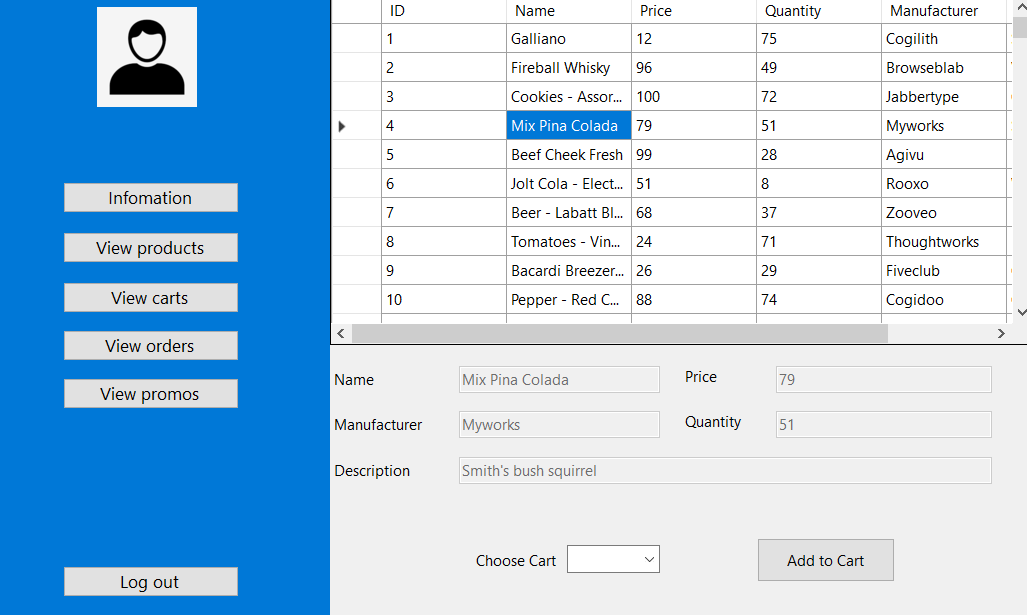
\includegraphics[height=0.4\textheight]{img/client_1.png}
	\caption{Демонстрация экрана клиентов при добавления товаров в корзину}
	\label{img:ex10}
\end{figure}

\clearpage
\section*{Создание базы данных}
\begin{lstlisting}[caption={Создание всех таблиц}, label={lst:createtable}]
	drop table userdb CASCADE;
	drop table promodb CASCADE;
	drop table productdb CASCADE;
	drop table userpromodb CASCADE;
	drop table cartdb CASCADE;
	drop table itemcartdb CASCADE;
	drop table orderdb CASCADE;
	drop table itemorderdb CASCADE;
	
	create table UserDB(
	Id serial primary key,
	Name varchar(50) not null,
	Phone varchar(50) not null,
	Address varchar(50) not null,
	Email varchar(50) not null,
	Login varchar(50) not null,
	Password varchar(50) not null,
	Role varchar(50) not null
	);
	
	create table PromoDB(
	Id serial primary key,
	code varchar(20) not null,
	discount int not null,
	data_start date not null,
	data_end date not null
	);
	create table ProductDB (
	Id serial primary key,
	Name varchar(50) not null,
	Price int not null,
	Quantity int not null,
	Manufacturer varchar(50) not null,
	Description varchar(50) not null
	);
	create table UserPromoDB(
	ID serial primary key,
	id_user int not null,
	id_promo int not null,
	foreign key (id_user) references UserDB(Id) ON DELETE CASCADE,
	foreign key (id_promo) references PromoDB(Id) ON DELETE CASCADE
	);
	
	create table CartDB(
	Id serial primary key,
	data_created date not null,
	id_user int references UserDB(Id) ON DELETE CASCADE
	);
	
	create table ItemCartDB(
	Id serial primary key,
	id_product int not null,
	id_cart int not null,
	quantity int not null,
	foreign key (id_cart) references CartDB(Id) ON DELETE CASCADE,
	foreign key (id_product) references ProductDB(Id) ON DELETE CASCADE
	);
	
	create table orderDB(
	Id serial primary key,
	status varchar(20) not null,
	data_created date not null,
	id_user int not null,
	id_promo int references PromoDB(Id) ON DELETE CASCADE,
	foreign key (id_user) references UserDB(Id) ON DELETE CASCADE
	);
	
	create table ItemOrderDB(
	Id serial primary key,
	id_product int not null,
	id_order int not null,
	quantity int not null,
	foreign key (id_order) references OrderDB(Id) ON DELETE CASCADE,
	foreign key (id_product) references ProductDB(Id) ON DELETE CASCADE
	);
\end{lstlisting}

\begin{lstlisting}[caption={Реализация триггера}, label={lst:trigger}]
	drop trigger after_itemorder_insert on itemorderdb;
	
	create or replace function process_itemorder()
	returns trigger
	as
	$$
	begin
	update productdb set quantity = (select quantity - new.quantity from productdb where id = new.id_product) where id = new.id_product;
	RETURN NEW;
	
	end;
	$$	LANGUAGE plpgsql;
	
	CREATE TRIGGER after_itemorder_insert
	AFTER INSERT ON itemorderdb
	for each row
	EXECUTE FUNCTION process_itemorder();
\end{lstlisting}

\begin{lstlisting}[caption={Создание роли администратора и выдыча права}, label={lst:role1}]
	create role Radmin with
	connection limit -1
	login
	password 'admin';
	
	grant all privileges
	on all tables in schema public
	to Radmin;
\end{lstlisting}

\begin{lstlisting}[caption={Создание роли поставщика и выдыча права}, label={lst:role2}]
	create role Rseller with
	connection limit 2
	login
	password 'seller';
	
	grant select on
	public."productdb",
	public."orderdb",
	public."userdb"
	to Rseller;
	
	grant insert on
	public."productdb"
	to Rseller;
	
	grant update on
	public."productdb",
	public."orderdb",
	public."itemorderdb",
	public."userdb"
	to Rseller;
	
	grant delete on
	public."productdb",
	public."orderdb",
	public."itemorderdb"
	to Rseller;
\end{lstlisting}

\begin{lstlisting}[caption={Создание роли клиента и выдыча права}, label={lst:role4}]
	create role Rclient with
	connection limit 100
	login
	password 'client';
	
	grant select on 
	public."productdb",
	public."cartdb",
	public."itemcartdb", 
	public."orderdb",
	public."itemorderdb",
	public."userdb"
	to Rclient;
	
	grant insert on
	public."cartdb",
	public."itemcartdb", 
	public."orderdb",
	public."itemorderdb"
	to Rclient;	
	
	grant update on
	public."cartdb",
	public."itemcartdb", 
	public."orderdb",
	public."itemorderdb",
	public."userdb"
	to Rclient;
	
	grant delete on
	public."cartdb",
	public."itemcartdb"
	to Rclient;
\end{lstlisting}

\begin{lstlisting}[caption={Создание роли гости и выдыча права}, label={lst:role5}]
	create role Rguest with
	connection limit 100
	login
	password 'guest';
	
	grant insert on
	public."userdb"
	to Rguest;	
	
\end{lstlisting}


\begin{lstlisting}[caption={Реализация тестирования для триггера after\_itemorder\_insert}, label={lst:test2}]
	CREATE OR REPLACE FUNCTION test_trigger(product_id int, 
	order_id int, quantityI int)
	RETURNS void AS $$
	DECLARE
	quantity_after int;
	quantity_before int;
	BEGIN
	select quantity into quantity_before from productdb 
	where id = product_id;
	
	INSERT INTO itemorderdb(id_product, id_order, quantity) 
	VALUES (product_id, order_id, quantityI);
	
	SELECT quantity INTO quantity_after FROM
	productdb WHERE id = product_id;
	
	if (quantity_after  = quantity_before - quantityI) then
	RAISE NOTICE 'This test passed';
	else 
	RAISE EXCEPTION 'Test failed';
	end if;
	END;
	$$ LANGUAGE plpgsql;
	
	-- Запуск теста
	SELECT test_trigger(1, 1, 5);
	SELECT test_trigger(2, 1, 5);
	SELECT test_trigger(3, 1, 5);
	
\end{lstlisting}

\begin{lstlisting}[caption={Функция входа в систему }, label={lst:pro1}]
	private void btnSignIn_Click(object sender, EventArgs e)
	{
		try
		{
			string login = tbUsername.Text;
			string password = tbPassword.Text;
			if (login == "" || password == "")
			{
				throw new Exception("Input error");
			}
			User user = _userService.LogIn(login, password);
			switch (user.Role)
			{
				case Role.Admin:
				FormAdmin frm_admin = new FormAdmin(user.Id, _userService, 
				_productService, _promoService, _orderService, _cartService,
				_itemOrderService, _itemCartService);
				frm_admin.ShowDialog(this);
				break;
				case Role.Seller:
				FormSelller frm_seller = new FormSelller(user.Id, _userService,
				_productService, _promoService, _orderService, _cartService, 
				_itemOrderService, _itemCartService);
				frm_seller.ShowDialog(this);
				break;
				case Role.Client:
				FormClient frm_client = new FormClient(user.Id, _userService,
				_productService, _promoService, _orderService, _cartService,
				_itemOrderService, _itemCartService);
				frm_client.ShowDialog(this);
				break;
			}
			this.Close();
		}
		catch (Exception ex) { MessageBox.Show(ex.Message, "Error", MessageBoxButtons.OK,
			MessageBoxIcon.Error); }
	}
	
\end{lstlisting}

\begin{lstlisting}[caption={Функция работы поользователей}, label={lst:pro2}]
	public User GetUser(int id)
	{
		CheckConnection.checkConnection(Connector);
		string query = queryGetUser(id);
		
		NpgsqlCommand cmd = new NpgsqlCommand(query, Connector.Connect);
		
		User user = null;
		
		NpgsqlDataReader reader = cmd.ExecuteReader();
		if (reader.Read())
		{
			user = new User(reader.GetInt32(0), reader.GetString(1), reader.GetString(2),
			reader.GetString(3), reader.GetString(4), reader.GetString(5), reader.GetString(6), (Role)Enum.Parse(typeof(Role), reader.GetString(7)));
		}
		reader.Close();
		return user;
	}
	
	public User GetUser(string login)
	{
		CheckConnection.checkConnection(Connector);
		string query = queryGetUser(login);
		
		NpgsqlCommand cmd = new NpgsqlCommand(query, Connector.Connect);
		
		User user = null;
		NpgsqlDataReader reader = cmd.ExecuteReader();
		
		if (reader.Read())
		{
			user = new User(reader.GetInt32(0), reader.GetString(1), reader.GetString(2),
			reader.GetString(3), reader.GetString(4), reader.GetString(5), reader.GetString(6), (Role)Enum.Parse(typeof(Role), reader.GetString(7)));
		}
		reader.Close();
		
		return user;
	}
	
	public void AddUser(User user)
	{
		CheckConnection.checkConnection(Connector);
		string query = queryAddUser(user);
		NpgsqlCommand cmd = new NpgsqlCommand(query, Connector.Connect);
		cmd.ExecuteNonQuery();
	}
	public void DelUser(User user)
	{
		CheckConnection.checkConnection(Connector);
		string query = queryDelUser(user);
		NpgsqlCommand cmd = new NpgsqlCommand(query, Connector.Connect);
		cmd.ExecuteNonQuery();
	}
	public void UpdateUser(User user)
	{
		CheckConnection.checkConnection(Connector);
		string query = queryUpdateUser(user);
		NpgsqlCommand cmd = new NpgsqlCommand(query, Connector.Connect);
		cmd.ExecuteNonQuery();
	}
	
	public List<User> GetAll()
	{
		CheckConnection.checkConnection(Connector);
		string query = queryGetAll();
		List<User> allUser = new List<User>();
		NpgsqlCommand cmd = new NpgsqlCommand(query, Connector.Connect);
		using (NpgsqlDataReader reader = cmd.ExecuteReader())
		{
			while (reader.Read())
			{
				allUser.Add(new User(reader.GetInt32(0), reader.GetString(1), reader.GetString(2),
				reader.GetString(3), reader.GetString(4), reader.GetString(5), reader.GetString(6), (Role)Enum.Parse(typeof(Role), reader.GetString(7))));                  
			}
			reader.Close();
		}
		return allUser;
	}
	
	public int CountAllUsers()
	{
		CheckConnection.checkConnection(Connector);
		string query = queryCountAllUsers();
		
		NpgsqlCommand cmd = new NpgsqlCommand(query, Connector.Connect);
		
		return Convert.ToInt32(cmd.ExecuteScalar());
	}
	
\end{lstlisting}